\section{Additional results}
\label{app:sec:additional_exp}

\subsection{Baseline Comparison to More PEFT Methods}

We conduct additional comparison studies against more parameter-efficient fine-tuning methods, including IA3\cite{liu2022few}, DORA. \cite{liu2024dora}.  
\begin{table}[!t]
\centering

\caption{\textbf{Additional Comparison Experiment.} Normalized scores are in the parentheses.}
\vspace{-2mm}
\small
\begin{tabular}{llll}
\toprule
% Method & MATH & Humaneval & ARC-Challenge \\
\textbf{Method} & \textbf{GSM8K} & \textbf{MBPP-Pro} & \textbf{ARC-Easy} \\

\midrule
\llama & {\normalsize 75.89 {\footnotesize (\grey{1.00})}} & {\normalsize 64.65 {\footnotesize (\grey{1.00})}} & {\normalsize 88.59 {\footnotesize (\grey{1.00})}} \\
% \quad + LoRA & {\normalsize 70.58 {\footnotesize (\red{0.93})}} & {\normalsize 67.68 {\footnotesize (\green{1.05})}} & {\normalsize 88.97 {\footnotesize (\green{1.00})}} \\
\quad + IA3 & {\normalsize 78.01 {\footnotesize (\green{1.03})}} & {\normalsize \textbf{67.68} {\footnotesize (\green{\textbf{1.05}})}} & {\normalsize 89.10 {\footnotesize (\green{1.01})}} \\
\quad + DORA & {\normalsize 78.09 {\footnotesize (\green{1.03})}} & {\normalsize 64.65 {\footnotesize (\grey{1.00})}} & {\normalsize 89.14 {\footnotesize (\green{1.01})}} \\
\quad + SVF(Ours) & \textbf{{\normalsize 79.15 {\footnotesize (\green{1.04})}}} & {\normalsize 66.67 {\footnotesize (\green{1.03})}} & \textbf{{\normalsize 89.56 {\footnotesize (\green{1.01})}}} \\

\midrule

\textbf{Method} & \textbf{MATH} & \textbf{Humaneval} & \textbf{ARC-Challenge} \\

\midrule
\llama & {\normalsize 24.54 {\footnotesize (\grey{1.00})}} & {\normalsize 60.98 {\footnotesize (\grey{1.00})}} & {\normalsize 80.63 {\footnotesize (\grey{1.00})}} \\
% \quad + LoRA & {\normalsize 21.68 {\footnotesize (\red{0.88})}} & {\normalsize 52.44 {\footnotesize (\red{0.86})}} & {\normalsize 81.06 {\footnotesize (\green{1.01})}} \\
\quad + IA3 & {\normalsize 23.64 {\footnotesize (\red{0.96})}} & {\normalsize 59.76 {\footnotesize (\red{0.98})}} & {\normalsize 81.57 {\footnotesize (\green{1.01})}} \\
\quad + DORA & {\normalsize 24.44 {\footnotesize (\red{0.99})}} & {\normalsize 52.44 {\footnotesize (\red{0.86})}} & {\normalsize 81.14 {\footnotesize (\green{1.01})}} \\
\quad + \implname (Prompt) & {\normalsize 25.22 {\footnotesize (\green{1.03})}} & {\normalsize 61.59 {\footnotesize (\green{1.01})}} & {\normalsize 81.74 {\footnotesize (\green{1.01})}} \\
\quad + \implname (Cls-expert) & {\normalsize 25.18 {\footnotesize (\green{1.03})}} & {\normalsize 62.80 {\footnotesize (\green{1.03})}} & {\normalsize 81.37 {\footnotesize (\green{1.01})}} \\
\quad + \implname (Few-shot) & \textbf{{\normalsize 25.47 {\footnotesize (\green{1.04})}}} & \textbf{{\normalsize 62.99 {\footnotesize (\green{1.03})}}} & \textbf{{\normalsize 82.61 {\footnotesize (\green{1.02})}}} \\


\bottomrule

\end{tabular}

\label{tab:res:svf_additional_baselines}
\vspace{-4mm}
\end{table}


As Table~\ref{tab:res:svf_additional_baselines} shows, \svdacro still outperforms other methods and shows promising generalized performance.

\subsection{Impact from number of few-shots}
\label{app:sec:ablation_few_shots}


\begin{wraptable}{r}{0.5\textwidth}
\vspace{-4mm}
\caption{\textbf{Few-shot adaptation scaling.} Performance varies with number of examples.
}
% \vspace{-3.5mm}
\centering
\resizebox{0.45\textwidth}{!}{
\begin{tabular}{lc}
\toprule
\textbf{Method} & \textbf{ARC-Challenge} \\
\midrule
\llama & {\normalsize 80.63 {\footnotesize (\grey{1.00})}} \\
\midrule

\quad + 3-shot adaptation & {\normalsize 82.18 {\footnotesize (\green{1.02})}} \\
\quad + 5-shot adaptation & {\normalsize 82.38 {\footnotesize (\green{1.02})}} \\
\quad + 10-shot adaptation & \textbf{{\normalsize 82.61 {\footnotesize (\green{1.02})}}} \\
\quad + 20-shot adaptation & \textbf{{\normalsize 82.61 {\footnotesize (\green{1.02})}}} \\

\bottomrule
\end{tabular}}
\label{tab:ablation:few_shot_adaptation}
\vspace{-10mm}
\end{wraptable}


We investigate the relationship between the number of samples available for few-shot adaptation and downstream performance.
Our analysis focused on the test task where \llama demonstrates the highest baseline performance, to prevent the potential for a null signal in our CEM-based search.

As Table~\ref{tab:ablation:few_shot_adaptation} shows, substantial benefits of our few-shot strategy are evident with as few as 3 to 5 test samples.
Moreover, performance appears to plateau beyond 10 samples, underscoring how our essential and inherently regularized \svdacro parameterization effectively complements self-adaptation.
This efficiency enables optimal use of data to enhance understanding of the test task.

For completeness, we have also conducted experiments with identical settings on IA$^3$~\citep{liu2022few}, another method that leverages few-shot examples.
All experiments were conducted with full batch size, a learning rate of $5 \times 10^{-5}$, with 100 and 1000 training steps.

Our results indicate that the performance of IA$^3$ on the unseen test tasks is inferior to CEM-based adaptation for all numbers of few shots considered.
We note that in our experiment, we have to considerably limit the number of optimization steps to avoid overfitting the 500,000 parameters of IA$^3$ on the few-shot samples. However, we believe overfitting might still be occurring to some degree even after only 100 steps, as also validated by the model’s perfect training accuracy on this extremely small dataset.
This limitation of fine-tuning-based adaptation highlights the superior generalization capability of our CEM-based adaptation approach in \implname.


\subsection{Cross-model svf transfer on the training tasks}
We provide complementary results to Table~\ref{tab:analysis:cross_model_main} in the main text, where we analyze the \svdacro cross-model transfer performance from training on GSM8K, MBPP-pro, and ARC-Easy to our considered test tasks. In Table~\ref{tab:analysis:cross_model_app}, we show the results in the same transfer setting this time evaluating \mistral on the same training tasks where the \llama \svdacro vectors were obtained from. Overall, we recognize a similar trend, albeit with less consistent improvement from the original model (only in 1 out of 3 tasks), but still much higher performance than the randomly shuffled baseline. These results further confirm that the canonical ordering of the \svdacro parameterization is key for cross-model transfer, highlighting once more its inherent suitability to empower self-adaptation.

\begin{table}[!h]
\caption{
\textbf{Cross-model $\boldsymbol{z}$ Vector Transfer.}
Results from transfering the SVF expert vectors trained on \llama to \mistral in the respective training tasks.}
\vspace{-3.5mm}
\centering
\begin{tabular}{lccc}
\toprule
\textbf{Method} & \textbf{GSM8K} & \textbf{MBPP-pro} & \textbf{ARC-Easy} \\
%\textit{SVF training task} & \small{\textit{GSM8K}} & \small{\textit{MBPP-pro}} & \small{\textit{ARC-Easy}} \\
\midrule

\textsc{Mistral-7B-Instruct-v0.3} & \textbf{{\normalsize 42.83 {\footnotesize (\grey{1.00})}}} & \textbf{{\normalsize 49.50 {\footnotesize (\grey{1.00})}}} & {\normalsize 81.65 {\footnotesize (\grey{1.00})}} \\

\midrule

\quad + Llama SVF (ordered $\sigma_i$) & {\normalsize 42.61 {\footnotesize (\red{0.99})}} & {\normalsize 48.48 {\footnotesize (\red{0.98})}} & \textbf{{\normalsize 81.78 {\footnotesize (\grey{1.00})}}} \\
\quad + Llama SVF (shuffled $\sigma_i$) & {\normalsize 41.93 {\footnotesize (\red{0.98})}} & {\normalsize 46.34 {\footnotesize (\red{0.94})}} & {\normalsize 80.81 {\footnotesize (\red{0.99})}} \\


\bottomrule
\end{tabular}
\label{tab:analysis:cross_model_app}
\end{table}

\subsection{Training curve of LoRA and policy gradient}

Figure~\ref{app:fig:lora_learning_curves} gives the learning curves for LoRA training on the GSM8K task.

\begin{figure}[h]
    \centering
    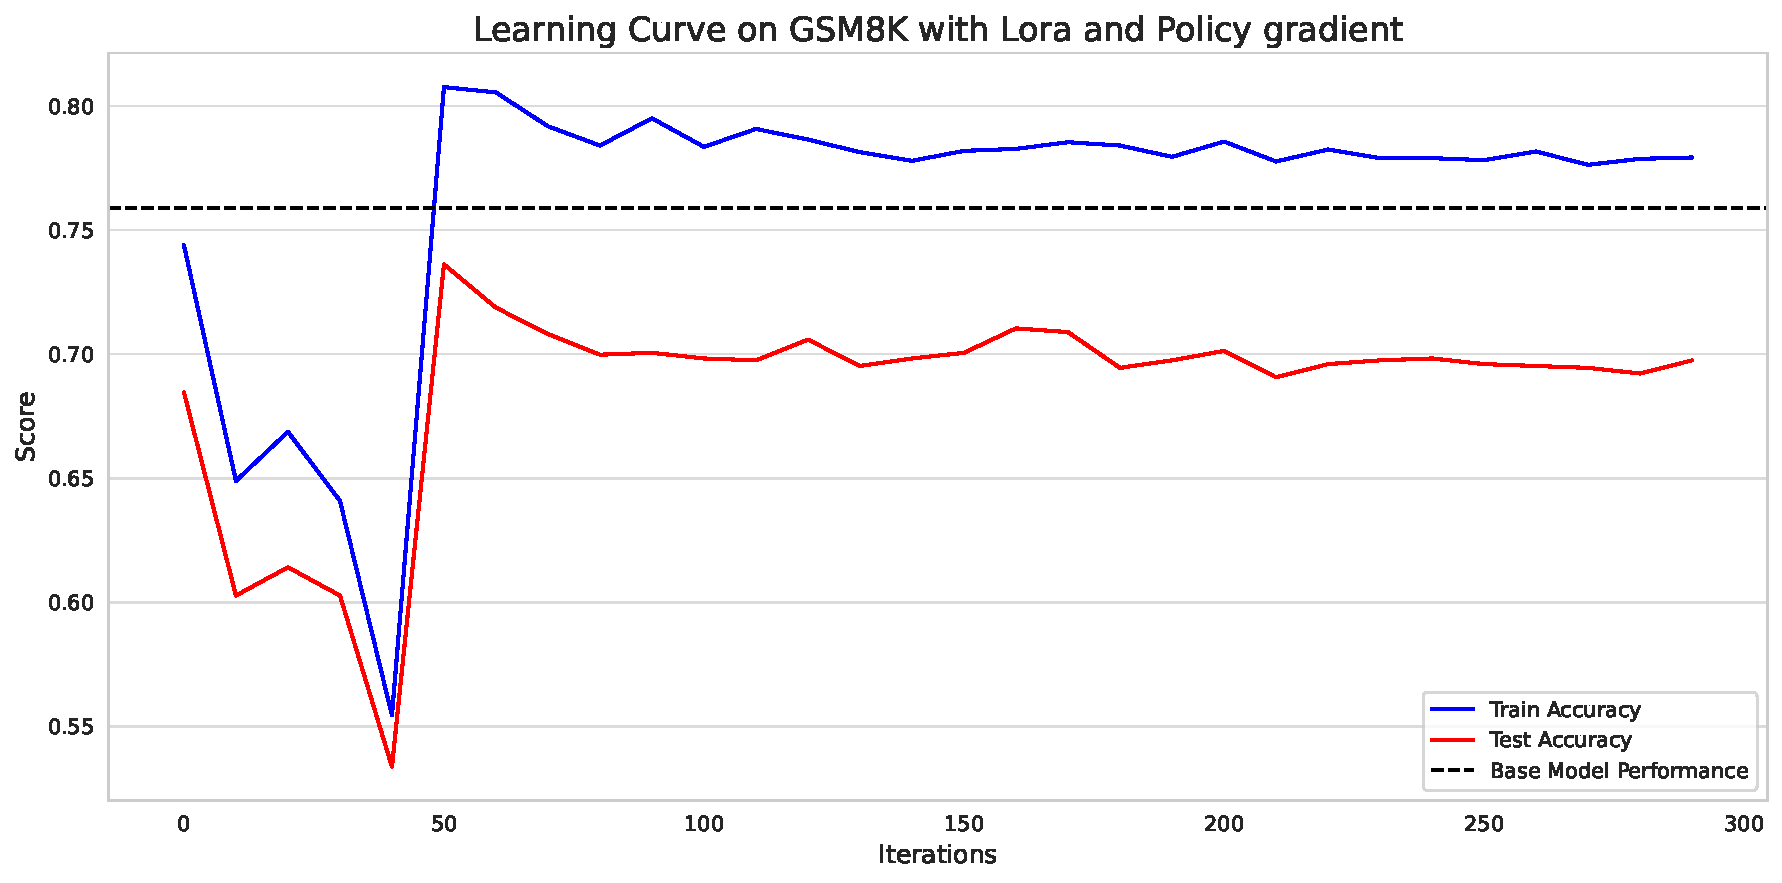
\includegraphics[width=0.6\textwidth]{images/lora_training_curve.pdf}
    \caption{\textbf{Training LoRA with policy gradient.} The dashed line shows the performance of \llama on the test split. LoRA collapses at the beginning of the training stage and fails to recover, leading to negative effects on test performance. We swept a wide range of learning rates $(2 \times 10^{-4}, 5 \times 10^{-4}, \dots, 2\times 10{-2}, 5\times 10^{-2})$, and all learning curves were similar to the one presented.}
    \label{app:fig:lora_learning_curves}
\end{figure}
